\chapter{Introdução}
\pagestyle{plain}

\section{Contextualização}

Foi discutido que a experimentação em Engenharia de Software (ES) tem se tornado fundamental para desenvolver e melhorar métodos e ferramentas, bem como melhorar os processos de manutenção de software \cite{kitchenham2007large}. Essa discussão permite que o conhecimento seja gerado de forma sistemática, disciplinada, quantificável e controlada \cite{wohlin2012experimentation}. Dessa forma melhora-se a qualidade dos experimentos \footnote[1]{Neste trabalho usaremos o termo "experimento" para denotar ambos os conceitos de "experimento controlado" e "\textit{quasi}-experimento controlado".} que por sua vez vem construir um corpo de conhecimento confiável e referente na área de experimentação em ES. 

Por outro lado, os sistemas de recomendação em ES vêm ganhado espaço por causa de própria evolução dos sistemas de recomendação tradicionais no mercado, como por exemplo Netflix, Spotify, Amazon, etc. Os sistemas de recomendação têm como objetivo recomendar algo mais atrativo para seu usuário, no caso de sistema de recomendação em ES o espaço de informação para gerar recomendação são os próprios recursos do ambiente de projeto e desenvolvimento de software, como código fonte, revisões do gerenciador de revisões de código e \textit{issues tracker} \cite{robillard2010recommendation}.

Dessa forma, acredita-se haver uma oportunidade de poder juntar essas duas áreas de pesquisa, na qual, será possível investigar o estudo de sistemas de recomendação para apresentar recomendações no contexto de experimentos e \textit{quasi}-experimentos controlados em LPS.

Atualmente, não há diretrizes específicas para avaliar a qualidade de experimentos em ES, especialmente, para áreas emergentes e em processo de consolidação como é o caso de Linha de Produto de Software (LPS), em que aspectos específicos do domínio como, por exemplo, os artefatos utilizados como objetos experimentais, a complexidade do treinamento, a dificuldade de seleção de participantes qualificados e a falta de repositórios, podem influenciar os experimentos. Além disso, tem-se percebido uma constante carência de documentação adequada dos experimentos que acabam por inviabilizar a repetição e auditoria dos estudos em LPS.

Realizar um experimento em LPS com qualidade, exige-se uma experiência considerável em ES e o mínimo de experiência em LPS. Com isso, a curva de aprendizado torna-se longa para extrair e apresentar de forma satisfatória, e com qualidade os resultados de experimentos em LPS. Além disso, a indústria tem adotado de forma crescente o conceito de LPS, desta forma, cada vez mais exigente por um corpo de conhecimento na área. Portanto, é um desafio para os estudantes e profissionais de ES poder realizar um experimento em LPS com qualidade.

Este trabalho propõe a especificação e implementação de um sistema de recomendação a fim de gerar recomendações de experimentos em LPS. Dessa forma, o usuário do sistema de recomendação terá processos e diretrizes confiáveis para a realização de seus experimentos em LPS. Espera-se que com estes processos e diretrizes os usuários possam planejar, executar, analisar e reportar experimentos em LPS, sendo assim, não comprometendo a replicação e auditoria dos mesmos.

\section{Motivação e Justificativa}
\label{sec:motivacao}
Realizar um experimento em LPS exige alguns pontos de atenção específicos para garantir a qualidade do experimento. Estes pontos tem sido investigados em um trabalho de mestrado em andamento do nosso Grupo de pesquisa em Reuso Sistemático de Software e Experimentação (GRSSE), neste trabalho vem sendo elaborado diretrizes para a determinar a qualidade de experimentos em LPS. Esta tarefa possui um árduo trabalho para garantir que, aspectos específicos do domínio como, por exemplo, os artefatos utilizados que são, os objetos experimentais, a complexidade do treinamento, a dificuldade de seleção de participantes qualificados em LPS e a falta de repositórios de LPS, não influenciem nos experimentos ao ponto de invalidá-los. A falta de experimentos com qualidade afeta diretamente a possibilidade de repetição dos estudos em LPS.

Sabendo que para realizar um experimento em LPS com qualidade exige-se seguir alguns modelos e diretrizes, construir um sistema de recomendação que recomende métodos, processos, diretrizes, entre outros, para realizar um experimento em LPS, pode proporcionar facilidade ao desenvolvimento dos mesmos, incentivando a cultura e desenvolvimento de experimentos na academia e industria.

Por meio do GRSSE, foi encontrada uma lacuna nas pesquisas de qualidade em experimentos de ES em LPS que proporciona esta pesquisa, apresentando um campo aberto à pesquisa para determinar qualidade e recomendação para experimentos em LPS.

\section{Objetivos}
\label{sec:objetivos}

Esta pesquisa tem como objetivo geral especificar e implementar um sistema de recomendação para experimentos em LPS caracterizados por sua qualidade

Os objetivos específicos deste projeto são:

\begin{itemize}
	\item gerar e representar um conjunto de meta dados a partir das informações sobre experimentos em LPS;
	\item definir técnicas de recomendação com base nos meta dados;
	\item projeto e desenvolvimento do sistema de recomendação e;
	\item avaliar e empacotar o sistema de recomendação.
\end{itemize}


\section{Metodologia de Desenvolvimento}
\label{sec:metodologia}

O processo de execução deste trabalho para chegar ao objetivo será, pesquisar de maneira exploratória um modelo de sistema de recomendação em experimentos de LPS. Para tal resultado será desenvolvido um projeto de software e em seguida executado o mesmo. A \ref{fig:metodologia_flow} apresenta as etapas de desenvolvimento desta pesquisa.

\begin{figure}[htb]
	\centering					
	{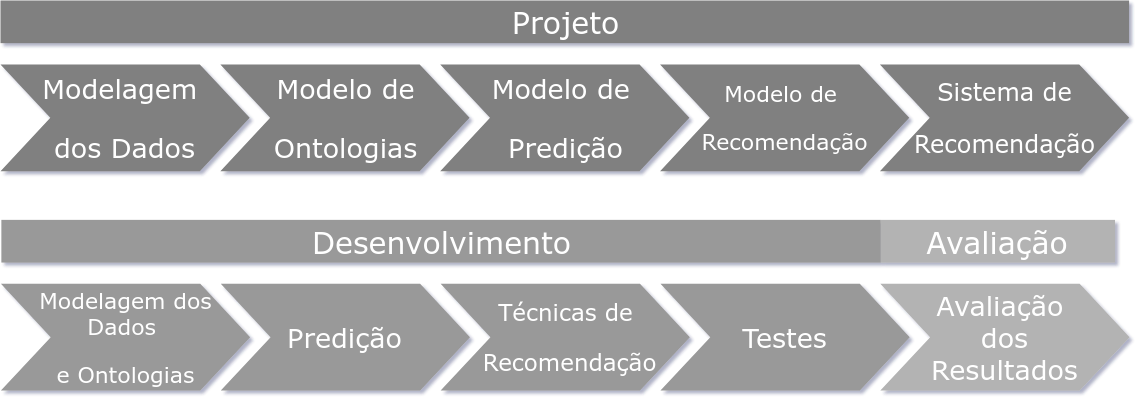
\includegraphics[scale=.4]{metodologia_flow.png}}
	
	\caption{Etapas da Metodologia de Desenvolvimento de Pesquisa}
	\label{fig:metodologia_flow}
\end{figure}

Neste projeto de pesquisa vamos levantar uma base de dados sobre a qualidade de experimentos em LPS. Por meio desta base será possível gerar um modelo de dados baseado em ontologias, \textbf{TBox} e \textbf{ABox}, com o objetivo de extrair informações preditivas desta base. Após processar essas informações baseada nos meta dados de qualidade de experimentos em LPS, será possível criar um sistema de recomendação, utilizando as ferramentas apropriadas de recomendação em ES.

\begin{itemize}
	\item \textbf{O Papel da Ontologia:} será de estruturar e modelar a base de informações extraída do Mapeamento Sistemático de experimentos em LPS que está sendo desenvolvido pelo GRSSE. Pode se dizer que este modelo será o conjunto de meta dados;
	
	\item \textbf{O Papel do Sistema de Recomendação:} será de interagir com o usuário afim de extrair informações relevantes, de modo que se possa determinando o deste perfil do usuário, para que possa ser realizada inferências no modelo ontológico de diretrizes de qualidade gerando recomendações de métodos, processos, diretrizes para o experimento do usuário.
\end{itemize}

O desenvolvimento do projeto, inclui realizar a escolha das tecnologias a serem usadas como ferramenta de construção do software, como por exemplo, as linguagens de programação, o ambiente de desenvolvimento, a diagramação do projeto, os \textit{stakeholders} envolvidos no projeto, ferramentas de \textit{Application Lifecycle Management} (ALM) aplicadas ao escopo do projeto, escolha das abordagens de sistemas de recomendação, definição do modelo de ontologias, definição da base de dados para representação tanto, dos dados de origem (itens, usuários), quanto, para representação dos dados para apresentação e armazenamento dos resultados obtidos da recomendação. 

Após a definição do projeto de software, inicia-se o processo de desenvolvimento do sistema de recomendação. Com o auxílio de ferramentas de ALM será possível acompanhar por todos os \textit{stakeholders} envolvidos o desenvolvimento online da ferramenta, desta forma se tornando um processo mais colaborativo entre eles. Inicialmente será realizado a modelagem dos dados extraído da avaliação de qualidade dos experimentos em LPS realizado pelo trabalho do GRSSE, que são 174 experimentos encontrado na literatura nesse ramo de pesquisa. Em seguida será aplicado um modelo de ontologia definido no projeto de software, nesta base de informações de experimentos, tem como propósito, realizar predições para um modelo mais abstrato sobre qualidade de experimentos em LPS. Na sequência será desenvolvido o modelo de recomendação, este desenvolvimento consiste na modelagem dos dados encontrado na predição da ontologia para extrair as informações necessárias para o modelo de recomendação, posteriormente aplicar os algoritmos neste modelo. Em seguida será desenvolvido um \textit{front-end} de interação com o usuário poder dar entrada na informações iniciais para gerar as recomendações. O último passo será realizado um estudo para avaliação deste sistema de recomendação.

\begin{figure}[htb]
	\centering					
	{
\includegraphics[scale=.5]{RSSE-overview.png}}
	
	\caption{Modelagem geral da RSSE proposta}
	\label{fig:RSSE-overview}
\end{figure}

A \ref{fig:RSSE-overview} apresenta o conceito geral da metodologia deste projeto. Iniciando pela entrada dos usuários, depois extraímos as preferencias dele, e em seguida será feita a extração de informações de contexto utilizando a base de meta dados em LPS, para então fazer inferência nos itens (que são experimentos em LPS), por meio dessa inferência será obtido as recomendações.

Inicialmente, a entrada de dados dos usuários está sendo definido da seguinte forma:

\begin{itemize}
	\item Informações de LPS:
	\subitem Dominio;
	\subitem Sub-dominio;
	\subitem Tipos de artefatos e;
	\subitem Feature module.
	\item Experimentos
	\subitem filtrar por qualidade.
\end{itemize}

\subsection{Empacotamento}

Todo projeto está sendo versionado no Github pelo link: https://github.com/rickvig/pcc-pesquisa.


\section{Organização do texto}

Este documento está estruturado da seguinte forma: o Capítulo 2 apresenta a Fundamentação Teórica sobre Linha de Produto de Software, Experimentos e Quasi-Experimentos em Engenharia de Software, qualidade de experimentos e quasi-experimentos em Engenharia de Software, Ontologias e Sistemas de Recomendação tradicionais e Sistemas de Recomendação em ES; o Capítulo 3 apresenta uma Ontologia para Experimentos de LPS; e o Capítulo 4 apresenta as considerações finais acerca deste projeto de dissertação de mestrado.


